\section{MOS-Transistoren\skript{Kap. 5}}

\subsection{Allgemeine Begriffe und Formeln}

\begin{tabular}{|l|l|l|}
	\hline
	$V_T$			& Schwellenspannung		& Threshold Voltage
	\\ \hline
	$V_{DS,sat}$	& Sättigungsspannung	&
	\\ \hline
	$a_A$			& Early-Faktor			&
	\\ \hline
	$\lambda$		& Kanallängen Modulationsfaktor & $\lambda = \frac{1}{V_A}$ 
	\\ \hline
	$V_A$			& Early-Spannung		& $V_A \approx a_A \cdot L$
	\\ \hline
	$\Phi_t$		& Temperaturspannung	& $\Phi_t = V_{temp} = \frac{kT}{e} \quad k = 1.38 \cdot 10^{23} J/K \quad e=1.6 \cdot 10^{-19} C$
	\\ \hline
	$r_{DS}$		& Ausgangswiderstand	& $r_{DS} = \frac{1}{g_0} \approx \frac{\Delta V_{DS}}{\Delta I_D} \quad 
											  \text{oder} \quad r_{DS} = \frac{V_A + V_{DS}}{I_{D,real}} \approx \frac{V_A}{I_D} $
	\\ \hline
	
\end{tabular}

\subsection{Inversion}

\begin{tabular}{|l|l|l|}
	\hline
	\textbf{Arbeitsbereich}	& \textbf{Bedingung}					& \textbf{Sättigungspannung}
	\\ \hline
	weak inversion			& $0 < V_{GS} < V_T - 60mV$				& $V_{DS,sat} \approx 5\Phi_t \approx 130mV \quad \text{(bei } T = 300K \text{)}$
	\\ \hline
	moderate inversion		& $V_T - 60mV < V_{GS} < V_T + 160mV$	&
	\\ \hline
	strong inversion		& $V_T + 160mV < V_{GS} $				& $V_{DS,sat} = V_{GS} - V_T$
	\\ \hline
\end{tabular}


\subsection{Betriebsarten}
Achtung: Beim Bipolar Transistor wird der Bereich links der Sättigungsgrenze als Sättigungsbereich bezeichnet, beim MOS-Transistor ist es der Bereich
rechts der Sättigungsgrenze!

\begin{figure}[h]
	\centering
	\begin{subfigure}[b]{6cm}
		\centering
		{\begin{circuitikz}[american, european resistors]
	\draw (1.5,0) node[circ, name=G] {} node[right] {G};
	\draw (4,0) node[circ, name=D] {} node[right] {D};
	\draw (4,-2) node[circ, name=S] {} node[right] {S};
	\draw (0,-2) -- (S);
	\draw (G) -- +(-1.5,0);
	\draw (3,0) to[R=$r_{DS0}$] +(0,-2);
	\draw (0,-2) to[V] ++(0,2) ;
	\draw (0,-2) -- + (0,-0.2) node[ground] {};
	\draw (D) -- +(-1,0);
	\draw[->, thick] (-0.9, -0.2) -- +(0,-1.4) node[midway, left] {$V_{GS}$};
\end{circuitikz}}
		\caption{Widerstandsbetrieb}
	\end{subfigure} \qquad\qquad
	\begin{subfigure}[b]{7cm}
		\centering
		{\begin{circuitikz}[american, european resistors]
	\draw (1.5,0) node[circ, name=G] {} node[right] {G};
	\draw (5,0) node[circ, name=D] {} node[right] {D};
	\draw (5,-2) node[circ, name=S] {} node[right] {S};
	\draw (0,-2) -- (S);
	\draw (G) -- +(-1.5,0);
	\draw (4,0) to[R=$r_{DS}$] +(0,-2);
	\draw (3,0) to[I,mirror,l=$g_mV_{GS}$] +(0,-2);
	\draw (0,-2) to[V] ++(0,2) ;
	\draw (0,-2) -- + (0,-0.2) node[ground] {};
	\draw (D) -- ++(-1,0) to[short, i_=$I_D$] +(-1,0);
	\draw[->, thick] (-0.9, -0.2) -- +(0,-1.4) node[midway, left] {$V_{GS}$};
\end{circuitikz}}
		\caption{Stromquellenbetrieb}
	\end{subfigure}
	\caption{Ersatzschlatbilder MOS-Transistoren}
\end{figure}

\subsubsection{Ungesättigter Betrieb}
Bei $V_{DS} = 0$ verhält sich der Kanal wie ein Widerstand. Die Kennlinie ist eine Gerade durch den Ursprung. Je steiler diese Gerade ist, desto
kleiner ist der Widerstand $r_{DS}$.

\subsubsection{Gesättigter Betrieb}
Bei $V_{DS} \geq V_{DS,sat}$ verhält sich der Kanal wie eine Stromquelle. Wenn die Geraden horizontal verlaufen ist $r_{DS} = \infty$ und
es handelt sich um einen idealen Transistor. Beim realen Transistor steigen jedoch diese Geraden immer leicht an.
Der Anstieg entspricht dem \textbf{Ausgangsleitwert} $g_0$, respektive dem \textbf{Ausgangswiderstand} $r_{DS}$.
Andere Bezeichnungen: differentieller- , Kleinsignal-, dynamischer Ausgangswiderstand.
\[
	r_{DS} = \frac{1}{g_0} = \frac{dV_{DS}}{dI_{D}} \approx \frac{\Delta V_{DS}}{\Delta I_D}
\]



\subsection{Transferkennlinie}

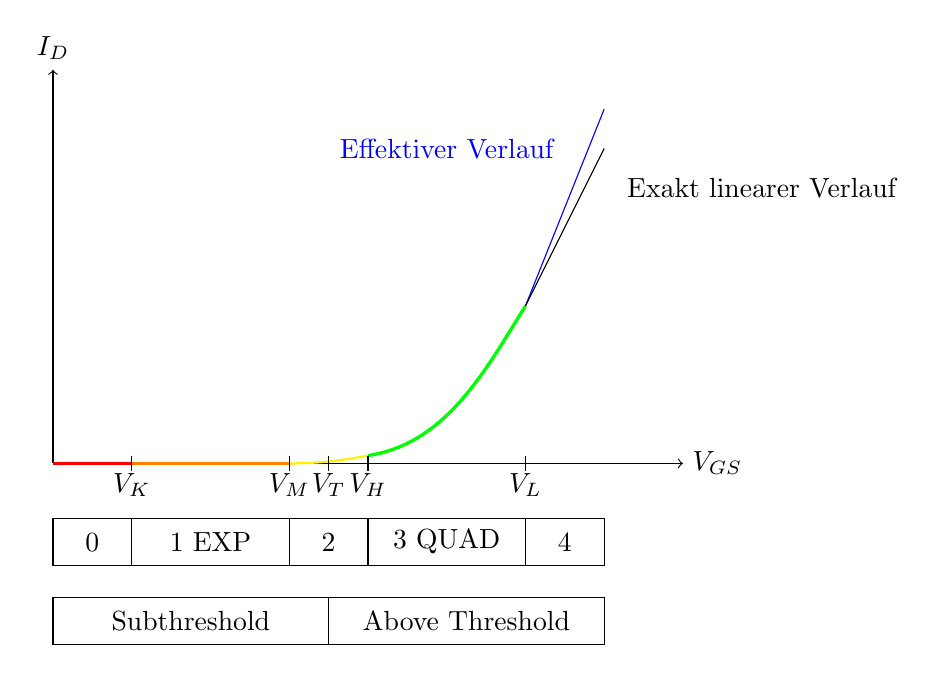
\begin{tikzpicture}

\draw [->] (0,0) -- (0,5) node [anchor=south] {$I_D$};
\draw [->] (0,0) -- (8,0) node [anchor=west] {$V_{GS}$};

\draw [color=red, thick] (0,0) -- (1,0);
\draw [color=orange, very thick] (1,0) -- (3,0);
\draw [color=yellow, thick] (3,0) arc (-90:-78:5);
\draw [color=green, very thick] (4.0,0.1) .. controls (5,0.25) and (5.5,1.2) .. (6,2);
\draw [color=blue] (6,2) -- (7,4.5);
\draw (6,2) -- (7,4);

\node [color=blue] at (5,4) {Effektiver Verlauf}; 
\node at (9,3.5) {Exakt linearer Verlauf};


\foreach \x in {1,3,4,6} {
	\draw (\x,0.1) -- (\x,-0.1);
	\draw (\x,-0.7) -- (\x,-1.3);
}

\draw (3.5,0.1) -- (3.5,-0.1);

\draw (0,-0.7) rectangle (7,-1.3);

\node at (1,0) [anchor=north] {$V_K$};
\node at (3,0) [anchor=north] {$V_M$};
\node at (3.5,0) [anchor=north] {$V_T$};
\node at (4,0) [anchor=north] {$V_H$};
\node at (6,0) [anchor=north] {$V_L$};

\node at (0.5,-1) {0};
\node at (2,-1) {1 EXP};
\node at (3.5,-1) {2};
\node at (5,-1) {3 QUAD};
\node at (6.5,-1) {4};

\draw (0,-1.7) rectangle (7,-2.3);
\draw (3.5,-1.7) -- (3.5,-2.3);
\node at (1.75,-2) {Subthreshold};
\node at (3.5+1.75,-2) {Above Threshold};
\end{tikzpicture}

\setArrayStretch{1.2}
\begin{tabular}{|lp{3cm}|p{6cm}|p{8cm}|}
	\hline
	& \textbf{Ausgangs\-strom\-bereich} & \textbf{Mathematische Charakterisierung} & \textbf{Zugrundeliegender physikalischer Effekt}
	\\ \hline
	\cellcolor{red!70}
	0 
	& Leckstrombereich (LECK) 
	& $I_D$ erreicht Minimalwert, der nicht weiter unterschritten werden kann
	& Drain-Substratdiode und Source-Substratdiode haben Leckströme im Substrat
	\\ \hline
	\cellcolor{orange!70}
	1
	& Exponentieller Bereich (EXP)
	& $I_D$ steigt exponentiell mit $V_{GS}$
	& Kanal zeigt schwache Inversion (Beim n-Kanal-Transistor: Ursprünglich p-leitender Kanal ist schwach n-leitend)
	\\ \hline
	\cellcolor{yellow!70}
	2
	& Schwellen Bereich (MOD)
	& Keine "`handlichen"' Formel für $I_D$ vorhanden
	& Kanal zeigt moderate Inversion (Kanalzustand liegt zwischen schwacher und starker Inversion)
	\\ \hline
	\cellcolor{green!70}
	3
	& Quadratischer Bereich (QUAD)
	& $I_D$ steigt quadratisch mit $V_{GS}$
	& Kanal zeigt starke Inversion (Beim n-Kanal-Transistor: Ursprünglich p-leitender Kanal wirk stark n-leitend)
	\\ \hline
	\cellcolor{blue!70}
	4
	& Linearer Bereich (LIN)
	& $I_D$ steigt annähernd linear mit $V_{GS}$ (halb QUAD, halb LIN)
	& Geschwindigkeitsänderung der Ladungsträger im Kanal (die Ladungsträger können nicht weiter beschleunigt werden)
	\\ \hline
\end{tabular}
\resetArrayStretch


\subsection{Drainstromgleichungen}
\begin{tabular}{|l|l|l|}
	\hline
		\textbf{Ausgangsstrom} 
		& \multicolumn{2}{c|}{\textbf{Ausgangsspannungsbereich} ($V_{DS}$-Bereich)}
	\\
		($I_D-, V_{GS}$-Bereich)
		& Transistor ungesättigt ($V_{DS} < V_{DS,sat}$)
		& Transistor gesättigt ($V_{DS} > V_{DS,sat}$)
	\\ \hline
		\multicolumn{3}{|c|}{\textbf{n-Kanal ohne Kanallängenmodulation und ohne unterschiedlicher Transkonduktanz:}}
	\\ \hline
		EXP-Bereich
		& $I_D = I_M e^{\frac{V_{GS}-V_M}{n_M \Phi_t}} (1-e^{\frac{-V_{DS}}{\Phi_t}})$
		& $I_D = I_M e^{\frac{V_{GS}-V_M}{n_M \Phi_t}}$
	\\ \hline
		QUAD-Bereich
		& $I_D = \beta [(V_{GS} - V_T) V_{DS} - \frac{V_{DS}^2}{2}]$
		& $I_D = \frac{\beta}{2}(V_{GS} - V_T)^2$
	\\ \hline
		\multicolumn{3}{|c|}{\textbf{n-Kanal mit Kanallängenmodulation und mit unterschiedlicher Transkonduktanz:}}
	\\ \hline
		EXP-Bereich
		& $I_D = I_M e^{\frac{V_{GS}-V_M}{n_M \Phi_t}} (1-e^{\frac{-V_{DS}}{\Phi_t}}) (1 + \lambda V_{DS})$
		& $I_D = I_M e^{\frac{V_{GS}-V_M}{n_M \Phi_t}} (1 + \lambda V_{DS})$
	\\ \hline
		QUAD-Bereich
		& $I_D = B [(V_{GS} - V_T) V_{DS} - \frac{V_{DS}^2}{2}] (1 + \lambda V_{DS})$
		& $I_D = \frac{\beta}{2}(V_{GS} - V_T)^2 (1 + \lambda V_{DS})$
	\\ \hline
		\multicolumn{3}{|c|}{\textbf{p-Kanal mit Kanallängenmodulation und mit unterschiedlicher Transkonduktanz:}}
	\\ \hline
		EXP-Bereich
		& $I_D = I_M e^{-\frac{V_{GS}-V_M}{n_M \Phi_t}} (1-e^{\frac{-V_{DS}}{\Phi_t}}) (1 - \lambda V_{DS})$
		& $I_D = I_M e^{-\frac{V_{GS}-V_M}{n_M \Phi_t}} (1 - \lambda V_{DS})$
	\\ \hline
		QUAD-Bereich
		& $I_D = -B [(V_{GS} - V_T) V_{DS} - \frac{V_{DS}^2}{2}] (1 - \lambda V_{DS})$
		& $I_D = -\frac{\beta}{2}(V_{GS} - V_T)^2 (1 - \lambda V_{DS})$
	\\ \hline
\end{tabular}
\newline

Die Sättigungsspannung beträgt im \textbf{EXP-Bereich} $5\Phi_t$, im \textbf{QUAD-Bereich} $V_{GS}-V_T$.

Parameter der Gleichungen:

\begin{tabularx}{\linewidth}{|l|l|X|}
	\hline
		$V_T$ & Schwellenspannung &
		Typisch $0.6V$ beim n-Kanal, resp. $-0.6V$ beim p-Kanal. $V_T$ ist stark von der Source-Bulk-Spannung abhängig (Body-Effekt):
		\[ 
			V_T = V_{T0} \pm \Delta V_T \quad \text{mit} \quad \Delta V_T = \gamma(\sqrt{V_SB \pm \Phi_0} -\sqrt{\Phi_0})
		\]
		positives Vorzeichen für n-Kanal, negatives für p-Kanal, $\gamma_N \approx 0.6\sqrt{V}$, $\gamma_P \approx 0.5\sqrt{V}$ 
	\\ \hline
		$\Phi_t$ & Temperaturspannung &
		\[
			\Phi_t = V_{Temp} = \frac{kT}{e} = 86.2 \frac{\mu V}{K}T
		\]
		somit ist $\Phi_t = 25.9mV$ bei $T=300^\circ K$ bzw. $27^\circ C$
	\\ \hline
		$I_M$ & Drainstrom &
		Drainstrom an der Grenze zwischen schwacher und moderater Inversion.
		\[
			I_M = \frac{W}{L} \cdot I_M'
		\]
		$I_M'$ ist der spezifische Drainstrom an der Grenze
	\\ \hline
		$n_M$ & Unterschwellen-Neigungsfaktor &
		Der Faktor $n_m$ ist von der Source-Bulk-Spannung $V_{SB}$ abhängig:
		\[
			n_M = 1 + \frac{\gamma}{2 \sqrt{V_{SB} + \Phi_0}}
		\]
		Für $V_{SB} = 0$ erhalten wir $n_M=1.39$. Häufig wird ein Wert von $n_M \approx 1.5$ angegeben.
	\\ \hline
		$\lambda$ & Kanallängen-Modulationsfaktor &
		inverser Wert der Early-Spannung
		\[
			\lambda = \frac{1}{V_A} \approx \frac{1}{a_A L}
		\]
		Der MOS-Transistor wird vielfach mit $\lambda = 0$ idealisiert, was die Handrechnung vereinfacht.
	\\ \hline
		$B, \beta$ & Transkondukdanz &
		Steilheit, Verstärkungsfaktor. Dieser Faktor ist im gesättigten und ungesättigten Betrieb \textbf{grundsätzlich verschieden}.
	\\ \hline
\end{tabularx}